\documentclass{article}\usepackage[]{graphicx}\usepackage[]{color}
% maxwidth is the original width if it is less than linewidth
% otherwise use linewidth (to make sure the graphics do not exceed the margin)
\makeatletter
\def\maxwidth{ %
  \ifdim\Gin@nat@width>\linewidth
    \linewidth
  \else
    \Gin@nat@width
  \fi
}
\makeatother

\definecolor{fgcolor}{rgb}{0.345, 0.345, 0.345}
\newcommand{\hlnum}[1]{\textcolor[rgb]{0.686,0.059,0.569}{#1}}%
\newcommand{\hlstr}[1]{\textcolor[rgb]{0.192,0.494,0.8}{#1}}%
\newcommand{\hlcom}[1]{\textcolor[rgb]{0.678,0.584,0.686}{\textit{#1}}}%
\newcommand{\hlopt}[1]{\textcolor[rgb]{0,0,0}{#1}}%
\newcommand{\hlstd}[1]{\textcolor[rgb]{0.345,0.345,0.345}{#1}}%
\newcommand{\hlkwa}[1]{\textcolor[rgb]{0.161,0.373,0.58}{\textbf{#1}}}%
\newcommand{\hlkwb}[1]{\textcolor[rgb]{0.69,0.353,0.396}{#1}}%
\newcommand{\hlkwc}[1]{\textcolor[rgb]{0.333,0.667,0.333}{#1}}%
\newcommand{\hlkwd}[1]{\textcolor[rgb]{0.737,0.353,0.396}{\textbf{#1}}}%
\let\hlipl\hlkwb

\usepackage{framed}
\makeatletter
\newenvironment{kframe}{%
 \def\at@end@of@kframe{}%
 \ifinner\ifhmode%
  \def\at@end@of@kframe{\end{minipage}}%
  \begin{minipage}{\columnwidth}%
 \fi\fi%
 \def\FrameCommand##1{\hskip\@totalleftmargin \hskip-\fboxsep
 \colorbox{shadecolor}{##1}\hskip-\fboxsep
     % There is no \\@totalrightmargin, so:
     \hskip-\linewidth \hskip-\@totalleftmargin \hskip\columnwidth}%
 \MakeFramed {\advance\hsize-\width
   \@totalleftmargin\z@ \linewidth\hsize
   \@setminipage}}%
 {\par\unskip\endMakeFramed%
 \at@end@of@kframe}
\makeatother

\definecolor{shadecolor}{rgb}{.97, .97, .97}
\definecolor{messagecolor}{rgb}{0, 0, 0}
\definecolor{warningcolor}{rgb}{1, 0, 1}
\definecolor{errorcolor}{rgb}{1, 0, 0}
\newenvironment{knitrout}{}{} % an empty environment to be redefined in TeX

\usepackage{alltt}
\usepackage{amsmath} %This allows me to use the align functionality.
                     %If you find yourself trying to replicate
                     %something you found online, ensure you're
                     %loading the necessary packages!
\usepackage{amsfonts}%Math font
\usepackage{graphicx}%For including graphics
\usepackage{hyperref}%For Hyperlinks
\hypersetup{colorlinks = true,citecolor=black}
\usepackage{natbib}        %For the bibliography
\bibliographystyle{apalike}%For the bibliography
\usepackage[margin=1.0in]{geometry}
\usepackage{float}
\IfFileExists{upquote.sty}{\usepackage{upquote}}{}
\begin{document}
\noindent \textbf{MA 354: Data Analysis I -- Fall 2021}\\%\\ gives you a new line
\noindent \textbf{Homework 3:}\vspace{1em}\\
\emph{Complete the following opportunities to use what we've talked about in class. These questions will be graded for correctness, communication and succinctness. Ensure you show your work and explain your logic in a legible and refined submission.}
%Comments -- anything after % is not put into the PDF
\begin{enumerate}
%%%%%%%%%%%%%%%%%%%%%%%%%%%%%%%%%%%%%%%%%%%%%%%%%%%%%%%%%%%%%%%%%%%%%%%%%%%%%%%
%%%%%%%%%%%%%%%%%%%%%%%%%%%%%%%%%%%%%%%%%%%%%%%%%%%%%%%%%%%%%%%%%%%%%%%%%%%%%%%
%%%%%%%%%  Question 0
%%%%%%%%%%%%%%%%%%%%%%%%%%%%%%%%%%%%%%%%%%%%%%%%%%%%%%%%%%%%%%%%%%%%%%%%%%%%%%%
%%%%%%%%%%%%%%%%%%%%%%%%%%%%%%%%%%%%%%%%%%%%%%%%%%%%%%%%%%%%%%%%%%%%%%%%%%%%%%%
\item[0.] \textbf{Complete weekly diagnostics.}
  
%%%%%%%%%%%%%%%%%%%%%%%%%%%%%%%%%%%%%%%%%%%%%%%%%%%%%%%%%%%%%%%%%%%%%%%%%%%%%%%
%%%%%%%%%%%%%%%%%%%%%%%%%%%%%%%%%%%%%%%%%%%%%%%%%%%%%%%%%%%%%%%%%%%%%%%%%%%%%%%
%%%%%%%%%  Question 1
%%%%%%%%%%%%%%%%%%%%%%%%%%%%%%%%%%%%%%%%%%%%%%%%%%%%%%%%%%%%%%%%%%%%%%%%%%%%%%%
%%%%%%%%%%%%%%%%%%%%%%%%%%%%%%%%%%%%%%%%%%%%%%%%%%%%%%%%%%%%%%%%%%%%%%%%%%%%%%%
\item Consider  data originally from a study of the nesting horseshoe crabs 
\citep{Brockmann96}. Each female crab in the study had a male crab attached to 
her in her nest. The study investigated factors that affect whether the female 
crab had any other males, called satellites, residing nearby her. Explanatory 
variables thought possibly to affect this included the female crab's color, 
spine condition, weight, and carapace width. The response outcome for each 
female crab is her number of satellites.
	 The sample is
	\begin{center}
		\begin{tabular}{|ccccccccccccccccc|}\hline
		 Number of Satellites& 0 & 1&  2&  3&  4&  5&  6&  7&  8&  9& 10& 11& 12& 13 &14& 15\\ \hline
		 Number of Observations&62& 16&  9& 19& 19& 15& 13&  4&  6&  3&  3&  1&  1&  1&  1&1\\\hline
 		\end{tabular}
	\end{center}
 	It is believed that the distribution of the number of satellites for a female 
 	crab is distributed Poisson$(\lambda)$ where the parameter $\lambda$ is of interest.
	\begin{enumerate}
	\item Calculate the method of moments estimator for $\lambda$.\\
	\textbf{Solution:}
\begin{knitrout}
\definecolor{shadecolor}{rgb}{0.969, 0.969, 0.969}\color{fgcolor}\begin{kframe}
\begin{alltt}
\hlkwd{library}\hlstd{(nleqslv)}
\hlcom{#put data into the dataframe}
\hlstd{crab.dat} \hlkwb{<-} \hlkwd{data.frame}\hlstd{(}\hlkwc{x}\hlstd{=}\hlkwd{c}\hlstd{(}\hlkwd{rep}\hlstd{(}\hlnum{0}\hlstd{,}\hlnum{62}\hlstd{),} \hlkwd{rep}\hlstd{(}\hlnum{1}\hlstd{,} \hlnum{16}\hlstd{),} \hlkwd{rep}\hlstd{(}\hlnum{2}\hlstd{,} \hlnum{9}\hlstd{),} \hlkwd{rep}\hlstd{(}\hlnum{3}\hlstd{,} \hlnum{19}\hlstd{),}
                           \hlkwd{rep}\hlstd{(}\hlnum{4}\hlstd{,} \hlnum{19}\hlstd{),} \hlkwd{rep}\hlstd{(}\hlnum{5}\hlstd{,} \hlnum{15}\hlstd{),} \hlkwd{rep}\hlstd{(}\hlnum{6}\hlstd{,} \hlnum{13}\hlstd{),} \hlkwd{rep}\hlstd{(}\hlnum{7}\hlstd{,} \hlnum{4}\hlstd{),}
                           \hlkwd{rep}\hlstd{(}\hlnum{8}\hlstd{,} \hlnum{6}\hlstd{),} \hlkwd{rep}\hlstd{(}\hlnum{9}\hlstd{,} \hlnum{3}\hlstd{),} \hlkwd{rep}\hlstd{(}\hlnum{10}\hlstd{,} \hlnum{3}\hlstd{),} \hlnum{11}\hlstd{,} \hlnum{12}\hlstd{,}
                           \hlnum{13}\hlstd{,} \hlnum{14}\hlstd{,} \hlnum{15}\hlstd{))}



\hlcom{#MOM function}
\hlstd{momfunc} \hlkwb{<-} \hlkwa{function}\hlstd{(}\hlkwc{par}\hlstd{,} \hlkwc{data}\hlstd{)\{}
  \hlstd{population.mean} \hlkwb{<-} \hlstd{par}
  \hlstd{sample.mean} \hlkwb{<-} \hlkwd{mean}\hlstd{(data)}
  \hlkwd{return}\hlstd{(sample.mean}\hlopt{-}\hlstd{population.mean)}
\hlstd{\}}

\hlstd{answer} \hlkwb{<-} \hlkwd{nleqslv}\hlstd{(}\hlkwc{x}\hlstd{=}\hlnum{1}\hlstd{,}
        \hlkwc{fn} \hlstd{= momfunc,}
        \hlkwc{data}\hlstd{=crab.dat}\hlopt{$}\hlstd{x)}

\hlstd{answer}\hlopt{$}\hlstd{x}
\end{alltt}
\begin{verbatim}
## [1] 2.977011
\end{verbatim}
\end{kframe}
\end{knitrout}
	\item Find the maximum likelihood estimator for $\lambda$.\\
	\textbf{Solution:}
\begin{knitrout}
\definecolor{shadecolor}{rgb}{0.969, 0.969, 0.969}\color{fgcolor}\begin{kframe}
\begin{alltt}
\hlstd{LLfunc} \hlkwb{<-} \hlkwa{function}\hlstd{(}\hlkwc{par}\hlstd{,} \hlkwc{data}\hlstd{)\{}
  \hlstd{answer} \hlkwb{<-} \hlkwd{sum}\hlstd{(}\hlkwd{dpois}\hlstd{(}\hlkwc{x}\hlstd{=data,} \hlkwc{lambda} \hlstd{= par,} \hlkwc{log}\hlstd{=T))}
  \hlopt{-}\hlstd{answer}
\hlstd{\}}

\hlstd{answer} \hlkwb{<-} \hlkwd{optim}\hlstd{(}\hlkwc{par} \hlstd{=} \hlnum{1}\hlstd{,}
      \hlkwc{fn} \hlstd{= LLfunc,}
      \hlkwc{data} \hlstd{= crab.dat}\hlopt{$}\hlstd{x,}
      \hlkwc{method} \hlstd{=} \hlstr{"Brent"}\hlstd{,}
      \hlkwc{lower} \hlstd{=} \hlnum{0}\hlstd{,}
      \hlkwc{upper} \hlstd{=} \hlnum{100}\hlstd{)}

\hlstd{answer}
\end{alltt}
\begin{verbatim}
## $par
## [1] 2.977011
## 
## $value
## [1] 505.4901
## 
## $counts
## function gradient 
##       NA       NA 
## 
## $convergence
## [1] 0
## 
## $message
## NULL
\end{verbatim}
\end{kframe}
\end{knitrout}
	\item Plot the data with the Poisson distribution fit with the MLE estimates. 
	How well does the distribution fit the data? 
\begin{knitrout}
\definecolor{shadecolor}{rgb}{0.969, 0.969, 0.969}\color{fgcolor}\begin{kframe}
\begin{alltt}
\hlkwd{library}\hlstd{(ggplot2)}
\hlkwd{library}\hlstd{(tidyverse)}
\end{alltt}


{\ttfamily\noindent\itshape\color{messagecolor}{\#\# -- Attaching packages --------------------------------------- tidyverse 1.3.1 --}}

{\ttfamily\noindent\itshape\color{messagecolor}{\#\# v tibble \ 3.1.2 \ \ \ \ v dplyr \ \ 1.0.7\\\#\# v tidyr \ \ 1.1.3 \ \ \ \ v stringr 1.4.0\\\#\# v readr \ \ 1.4.0 \ \ \ \ v forcats 0.5.1\\\#\# v purrr \ \ 0.3.4}}

{\ttfamily\noindent\itshape\color{messagecolor}{\#\# -- Conflicts ------------------------------------------ tidyverse\_conflicts() --\\\#\# x dplyr::filter() masks stats::filter()\\\#\# x dplyr::lag() \ \ \ masks stats::lag()}}\begin{alltt}
\hlstd{crab.dat.plot} \hlkwb{<-} \hlstd{crab.dat} \hlopt
  \hlkwd{mutate}\hlstd{(}\hlkwc{f} \hlstd{=} \hlkwd{dpois}\hlstd{(}\hlkwc{x}\hlstd{=x,} \hlkwc{lambda}\hlstd{=}\hlnum{2.977011}\hlstd{))}


\hlstd{sats} \hlkwb{<-} \hlnum{0}\hlopt{:}\hlnum{15}
\hlkwd{ggplot}\hlstd{(crab.dat.plot,} \hlkwd{aes}\hlstd{(}\hlkwc{x}\hlstd{=x))}\hlopt{+}
  \hlkwd{geom_histogram}\hlstd{(}\hlkwd{aes}\hlstd{(}\hlkwc{y}\hlstd{=..density..),} \hlkwc{fill}\hlstd{=}\hlstr{"deepskyblue2"}\hlstd{,} \hlkwc{color}\hlstd{=}\hlstr{"black"}\hlstd{,}
                 \hlkwc{binwidth}\hlstd{=}\hlnum{1}\hlstd{)}\hlopt{+}
  \hlkwd{geom_linerange}\hlstd{(}\hlkwd{aes}\hlstd{(}\hlkwc{ymin}\hlstd{=}\hlnum{0}\hlstd{,} \hlkwc{ymax}\hlstd{=f),} \hlkwc{color}\hlstd{=}\hlstr{"dark red"}\hlstd{)}\hlopt{+}
  \hlkwd{scale_x_continuous}\hlstd{(}\hlstr{"Number of satellites"}\hlstd{,}
                     \hlkwc{labels} \hlstd{=} \hlkwd{as.character}\hlstd{(sats),} \hlkwc{breaks} \hlstd{= sats)}\hlopt{+}
  \hlkwd{labs}\hlstd{(}\hlkwc{y}\hlstd{=}\hlstr{"Density"}\hlstd{,}
       \hlkwc{title}\hlstd{=}\hlstr{"Number of observations per satellite"}\hlstd{,}
       \hlkwc{subtitle}\hlstd{=}\hlstr{"Fitting Poisson distribution"}\hlstd{)}
\end{alltt}
\end{kframe}
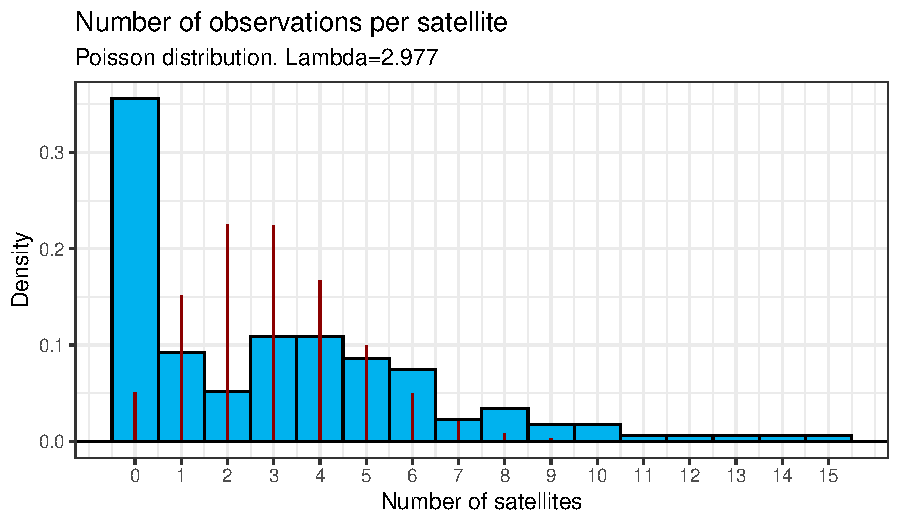
\includegraphics[width=\maxwidth]{figure/unnamed-chunk-3-1} 
\end{knitrout}
	\item Let's try another distribution - the zero-inflated Poisson distribution. 
	Now, it is believed that the distribution of the number of satellites for a 
	female crab is distributed Poisson$_0(\lambda,\sigma)$ where the parameters 
	$\lambda$ and $\sigma$ are of interest. Find the method of moments estimators 
	for both $\sigma$ and $\lambda$.
	 \[f_X(x|\lambda,\sigma)=(1-\sigma)\frac{\lambda^x e^{-\lambda}}{x!}I(x\geq1) 
	 + (\sigma+(1-\sigma)e^{-\lambda}) I(x=0)\]
	 \textbf{Hint:} Noticing that this is a function of the Poisson PMF and
	 rewriting it will help remarkably.\\
	 \textbf{Solution:}
\begin{knitrout}
\definecolor{shadecolor}{rgb}{0.969, 0.969, 0.969}\color{fgcolor}\begin{kframe}
\begin{alltt}
\hlstd{zip.pois} \hlkwb{<-} \hlkwa{function}\hlstd{(}\hlkwc{par}\hlstd{,} \hlkwc{data}\hlstd{)\{}
  \hlstd{lambda} \hlkwb{<-} \hlstd{par[}\hlnum{1}\hlstd{]}
  \hlstd{pi} \hlkwb{<-} \hlstd{par[}\hlnum{2}\hlstd{]}

  \hlstd{EX1} \hlkwb{<-} \hlstd{(}\hlnum{1}\hlopt{-}\hlstd{pi)}\hlopt{*}\hlstd{lambda}
  \hlstd{EX2} \hlkwb{<-} \hlstd{(}\hlnum{1}\hlopt{-}\hlstd{pi)}\hlopt{*}\hlstd{(lambda}\hlopt{^}\hlnum{2}\hlopt{+}\hlstd{lambda)}

  \hlstd{xbar1} \hlkwb{<-} \hlkwd{mean}\hlstd{(data)}
  \hlstd{xbar2} \hlkwb{<-} \hlkwd{mean}\hlstd{(data}\hlopt{^}\hlnum{2}\hlstd{)}

  \hlkwd{c}\hlstd{(EX1}\hlopt{-}\hlstd{xbar1, EX2}\hlopt{-}\hlstd{xbar2)}
\hlstd{\}}


\hlkwd{nleqslv}\hlstd{(}\hlkwc{x} \hlstd{=} \hlkwd{c}\hlstd{(}\hlnum{4.5}\hlstd{,}\hlnum{0.34}\hlstd{),} \hlcom{#best guess at parameter}
        \hlkwc{fn} \hlstd{= zip.pois,}
        \hlkwc{data} \hlstd{= crab.dat}\hlopt{$}\hlstd{x)}
\end{alltt}
\begin{verbatim}
## $x
## [1] 5.4633205 0.4550912
## 
## $fvec
## [1] 3.674039e-11 3.937686e-10
## 
## $termcd
## [1] 1
## 
## $message
## [1] "Function criterion near zero"
## 
## $scalex
## [1] 1 1
## 
## $nfcnt
## [1] 7
## 
## $njcnt
## [1] 1
## 
## $iter
## [1] 7
\end{verbatim}
\end{kframe}
\end{knitrout}
Let's graph the results to see how accurate this approach was! 

\begin{knitrout}
\definecolor{shadecolor}{rgb}{0.969, 0.969, 0.969}\color{fgcolor}\begin{kframe}
\begin{alltt}
\hlkwd{library}\hlstd{(}\hlstr{"VGAM"}\hlstd{)}
\end{alltt}


{\ttfamily\noindent\itshape\color{messagecolor}{\#\# Loading required package: stats4}}

{\ttfamily\noindent\itshape\color{messagecolor}{\#\# Loading required package: splines}}

{\ttfamily\noindent\itshape\color{messagecolor}{\#\# \\\#\# Attaching package: 'VGAM'}}

{\ttfamily\noindent\itshape\color{messagecolor}{\#\# The following object is masked from 'package:tidyr':\\\#\# \\\#\# \ \ \ \ fill}}\begin{alltt}
\hlstd{crab.dat.zim} \hlkwb{<-} \hlstd{crab.dat} \hlopt
          \hlkwd{mutate}\hlstd{(}\hlkwc{f} \hlstd{=} \hlkwd{dzipois}\hlstd{(}\hlkwc{x}\hlstd{=x,} \hlkwc{lambda}\hlstd{=}\hlnum{5.4633205}\hlstd{,} \hlkwc{pstr0}\hlstd{=}\hlnum{0.4550912}\hlstd{))}

\hlkwd{ggplot}\hlstd{(crab.dat.zim,} \hlkwd{aes}\hlstd{(}\hlkwc{x}\hlstd{=x))}\hlopt{+}
          \hlkwd{geom_histogram}\hlstd{(}\hlkwd{aes}\hlstd{(}\hlkwc{y}\hlstd{=..density..),} \hlkwc{fill}\hlstd{=}\hlstr{"deepskyblue2"}\hlstd{,} \hlkwc{color}\hlstd{=}\hlstr{"black"}\hlstd{,}
                         \hlkwc{binwidth}\hlstd{=}\hlnum{1}\hlstd{)}\hlopt{+}
          \hlkwd{geom_linerange}\hlstd{(}\hlkwd{aes}\hlstd{(}\hlkwc{ymin}\hlstd{=}\hlnum{0}\hlstd{,} \hlkwc{ymax}\hlstd{=f),} \hlkwc{color}\hlstd{=}\hlstr{"dark red"}\hlstd{)}\hlopt{+}
          \hlkwd{scale_x_continuous}\hlstd{(}\hlstr{"Number of satellites"}\hlstd{,}
                             \hlkwc{labels} \hlstd{=} \hlkwd{as.character}\hlstd{(sats),} \hlkwc{breaks} \hlstd{= sats)}\hlopt{+}
          \hlkwd{labs}\hlstd{(}\hlkwc{y}\hlstd{=}\hlstr{"Density"}\hlstd{,}
               \hlkwc{title}\hlstd{=}\hlstr{"Number of observations per satellite"}\hlstd{,}
               \hlkwc{subtitle}\hlstd{=}\hlstr{"Fitting Poisson distribution"}\hlstd{)}
\end{alltt}
\end{kframe}
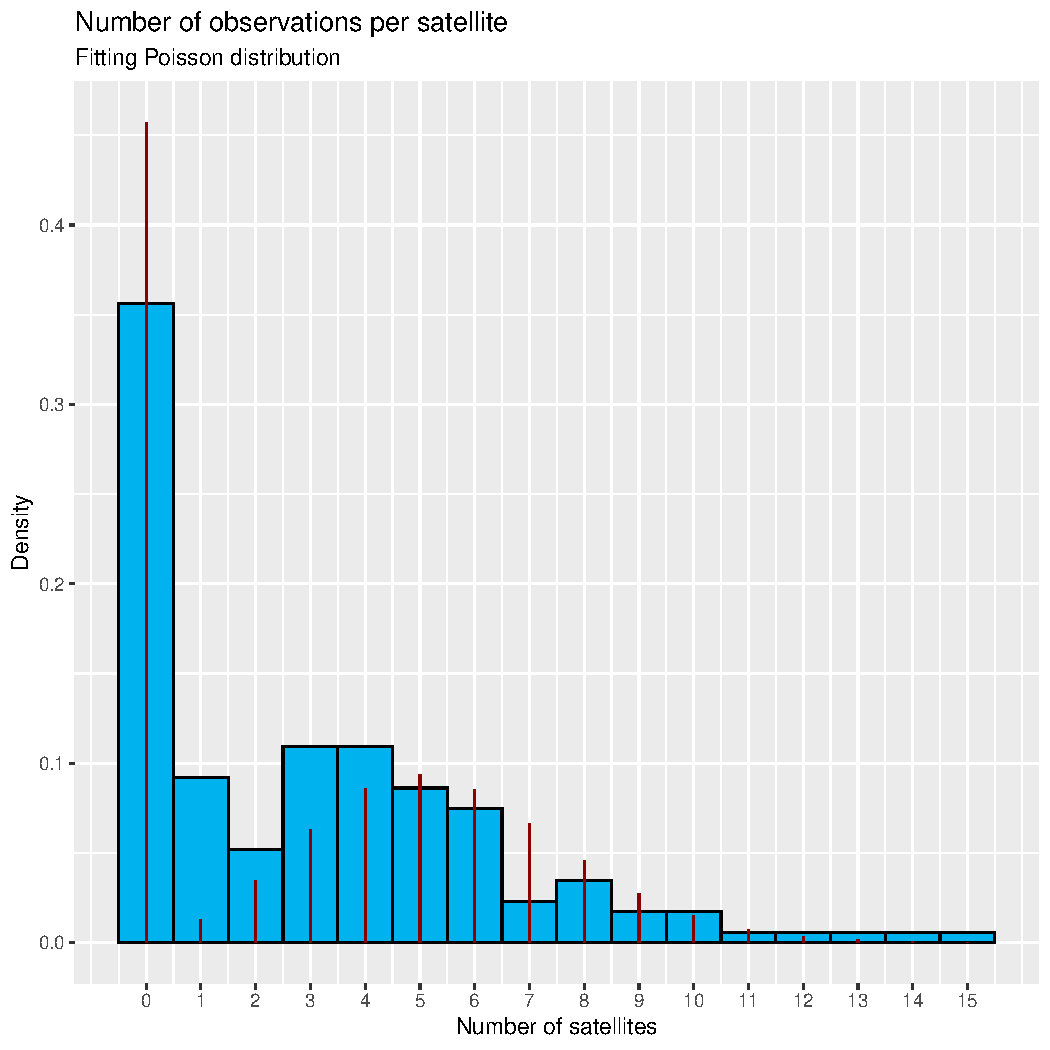
\includegraphics[width=\maxwidth]{figure/unnamed-chunk-5-1} 
\end{knitrout}
It would appear that MOM inflates zero too much, and underestimates the other values.

	 \item Find the maximum likelihood estimator for $\lambda$ and $\sigma$.
\begin{knitrout}
\definecolor{shadecolor}{rgb}{0.969, 0.969, 0.969}\color{fgcolor}\begin{kframe}
\begin{alltt}
\hlkwd{library}\hlstd{(Rfast)}
\end{alltt}


{\ttfamily\noindent\itshape\color{messagecolor}{\#\# Loading required package: Rcpp}}

{\ttfamily\noindent\itshape\color{messagecolor}{\#\# Loading required package: RcppZiggurat}}

{\ttfamily\noindent\itshape\color{messagecolor}{\#\# \\\#\# Attaching package: 'Rfast'}}

{\ttfamily\noindent\itshape\color{messagecolor}{\#\# The following object is masked from 'package:VGAM':\\\#\# \\\#\# \ \ \ \ Rank}}

{\ttfamily\noindent\itshape\color{messagecolor}{\#\# The following object is masked from 'package:dplyr':\\\#\# \\\#\# \ \ \ \ nth}}

{\ttfamily\noindent\itshape\color{messagecolor}{\#\# The following objects are masked from 'package:purrr':\\\#\# \\\#\# \ \ \ \ is\_integer, transpose}}\begin{alltt}
\hlkwd{zip.mle}\hlstd{(crab.dat}\hlopt{$}\hlstd{x)}
\end{alltt}
\begin{verbatim}
## $iters
## [1] 5
## 
## $loglik
## [1] -389.4734
## 
## $param
##    lambda        pi 
## 4.5774500 0.3496354
\end{verbatim}
\begin{alltt}
\hlcom{#MLE}
\hlstd{dpois.ll}\hlkwb{<-}\hlkwa{function}\hlstd{(}\hlkwc{par}\hlstd{,} \hlkwc{data}\hlstd{,} \hlkwc{neg}\hlstd{=T)\{}
  \hlstd{lambda} \hlkwb{<-} \hlstd{par[}\hlnum{1}\hlstd{]}
  \hlstd{pi} \hlkwb{<-} \hlstd{par[}\hlnum{2}\hlstd{]}
  \hlstd{ll} \hlkwb{<-} \hlkwd{sum}\hlstd{(}\hlkwd{dzipois}\hlstd{(}\hlkwc{x}\hlstd{=data,} \hlkwc{lambda}\hlstd{=lambda,} \hlkwc{pstr0}\hlstd{=pi,} \hlkwc{log}\hlstd{=T))}
  \hlkwd{ifelse}\hlstd{(neg,} \hlopt{-}\hlstd{ll, ll)}
\hlstd{\}}

\hlkwd{optim}\hlstd{(}\hlkwc{par} \hlstd{=} \hlkwd{c}\hlstd{(}\hlnum{1}\hlstd{,}\hlnum{0}\hlstd{),}
      \hlkwc{fn} \hlstd{= dpois.ll,}
      \hlkwc{data}\hlstd{=crab.dat}\hlopt{$}\hlstd{x)}
\end{alltt}
\begin{verbatim}
## $par
## [1] 4.5770922 0.3496381
## 
## $value
## [1] 389.4734
## 
## $counts
## function gradient 
##       71       NA 
## 
## $convergence
## [1] 0
## 
## $message
## NULL
\end{verbatim}
\end{kframe}
\end{knitrout}
	\item Plot a histogram of the data with the zero-inflated Poisson distribution
	fit with the MLE estimates. How well does the distribution fit the data?
\begin{knitrout}
\definecolor{shadecolor}{rgb}{0.969, 0.969, 0.969}\color{fgcolor}\begin{kframe}
\begin{alltt}
\hlstd{crab.dat.zim} \hlkwb{<-} \hlstd{crab.dat} \hlopt
  \hlkwd{mutate}\hlstd{(}\hlkwc{f} \hlstd{=} \hlkwd{dzipois}\hlstd{(}\hlkwc{x}\hlstd{=x,} \hlkwc{lambda}\hlstd{=}\hlnum{4.5770923}\hlstd{,} \hlkwc{pstr0}\hlstd{=}\hlnum{0.3496381}\hlstd{))}

\hlkwd{ggplot}\hlstd{(crab.dat.zim,} \hlkwd{aes}\hlstd{(}\hlkwc{x}\hlstd{=x))}\hlopt{+}
  \hlkwd{geom_histogram}\hlstd{(}\hlkwd{aes}\hlstd{(}\hlkwc{y}\hlstd{=..density..),} \hlkwc{fill}\hlstd{=}\hlstr{"deepskyblue2"}\hlstd{,} \hlkwc{color}\hlstd{=}\hlstr{"black"}\hlstd{,}
                 \hlkwc{binwidth}\hlstd{=}\hlnum{1}\hlstd{)}\hlopt{+}
  \hlkwd{geom_linerange}\hlstd{(}\hlkwd{aes}\hlstd{(}\hlkwc{ymin}\hlstd{=}\hlnum{0}\hlstd{,} \hlkwc{ymax}\hlstd{=f),} \hlkwc{color}\hlstd{=}\hlstr{"dark red"}\hlstd{)}\hlopt{+}
  \hlkwd{scale_x_continuous}\hlstd{(}\hlstr{"Number of satellites"}\hlstd{,}
                     \hlkwc{labels} \hlstd{=} \hlkwd{as.character}\hlstd{(sats),} \hlkwc{breaks} \hlstd{= sats)}\hlopt{+}
  \hlkwd{labs}\hlstd{(}\hlkwc{y}\hlstd{=}\hlstr{"Density"}\hlstd{,}
       \hlkwc{title}\hlstd{=}\hlstr{"Number of observations per satellite"}\hlstd{,}
       \hlkwc{subtitle}\hlstd{=}\hlstr{"Fitting Poisson distribution"}\hlstd{)}
\end{alltt}
\end{kframe}
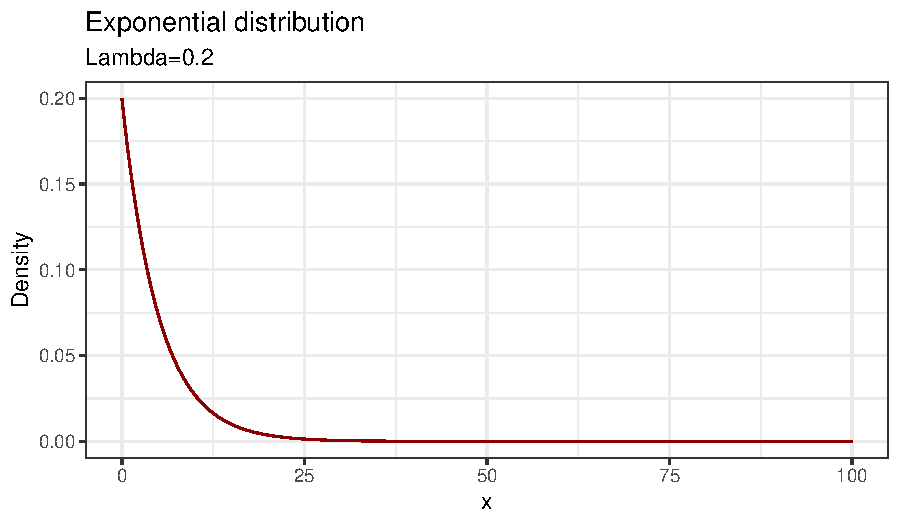
\includegraphics[width=\maxwidth]{figure/unnamed-chunk-7-1} 
\end{knitrout}
	\end{enumerate}
\newpage
%%%%%%%%%%%%%%%%%%%%%%%%%%%%%%%%%%%%%%%%%%%%%%%%%%%%%%%%%%%%%%%%%%%%%%%%%%%%%%%
%%%%%%%%%%%%%%%%%%%%%%%%%%%%%%%%%%%%%%%%%%%%%%%%%%%%%%%%%%%%%%%%%%%%%%%%%%%%%%%
%%%%%%%%%  Question 2
%%%%%%%%%%%%%%%%%%%%%%%%%%%%%%%%%%%%%%%%%%%%%%%%%%%%%%%%%%%%%%%%%%%%%%%%%%%%%%%
%%%%%%%%%%%%%%%%%%%%%%%%%%%%%%%%%%%%%%%%%%%%%%%%%%%%%%%%%%%%%%%%%%%%%%%%%%%%%%%
\item The time to death for rats injected with a toxic substance, denoted by $Y$
	(measured in days), follows an exponential distribution with $\lambda = 1/5$. That is,
	\[Y \sim \textrm{exponential}(\lambda = 1/5).\]
	This is the population distribution. It describes the time to death for all individual rats in the population.

  The \textbf{exponential distribution} serves as a very good model for measurements like waiting times or lifetimes.
  \begin{align*}
  \lambda &\in \mathbb{R^+}  \tag*{\textbf{[Parameters]}}\\
  \mathcal{X}&= \{\omega: \omega \in \mathbb{R^+}\} \tag*{\textbf{[Support]}}\\
  f_X(x|\mu,\sigma) &= \lambda e^{-\lambda x}~ I(x \in \mathbb{R^+}) \tag*{\textbf{[PDF]}}\\
  F_X(x|\mu,\sigma) &= \left(1- e^{-\lambda x}\right)I(x \in \mathbb{R^+}\tag*{\textbf{[CDF]}}\\
  F_X^{-1}(p|\mu,\sigma) &= \frac{-\ln(1-p)}{\lambda} \tag*{\textbf{[Inverse CDF]}}\\
  E(X) &= \frac{1}{\lambda} \tag*{\textbf{[Expected Value]}}\\
  var(X) &= \frac{1}{\lambda^2}\tag*{\textbf{[Population Variance]}}\\
  \end{align*}
	\begin{enumerate}
	  \item Plot the exponential$(\lambda = 1/5)$ population distribution.
\begin{knitrout}
\definecolor{shadecolor}{rgb}{0.969, 0.969, 0.969}\color{fgcolor}\begin{kframe}
\begin{alltt}
\hlstd{x}\hlkwb{<-}\hlkwd{seq}\hlstd{(}\hlnum{0}\hlstd{,} \hlnum{100}\hlstd{,} \hlnum{0.1}\hlstd{)}
\hlstd{y}\hlkwb{<-}\hlkwd{dexp}\hlstd{(x,} \hlnum{1}\hlopt{/}\hlnum{5}\hlstd{)}
\hlstd{ggdat}\hlkwb{<-}\hlkwd{data.frame}\hlstd{(x,y)}

\hlkwd{ggplot}\hlstd{(ggdat,} \hlkwd{aes}\hlstd{(}\hlkwc{x}\hlstd{=x,} \hlkwc{y}\hlstd{=y))}\hlopt{+}
  \hlkwd{geom_line}\hlstd{()}
\end{alltt}
\end{kframe}
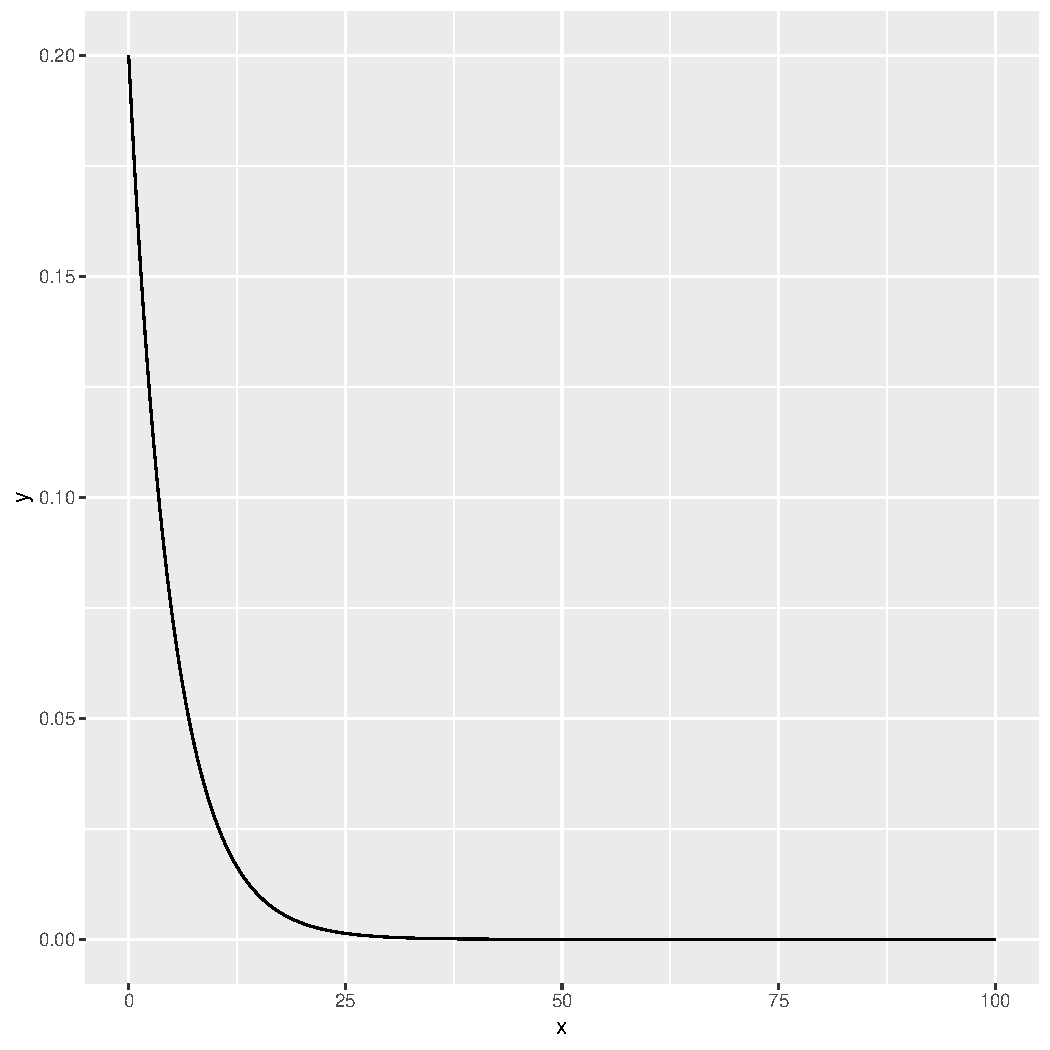
\includegraphics[width=\maxwidth]{figure/unnamed-chunk-8-1} 
\end{knitrout}
	  \item Mathematical statisticians can show the exact sampling distributions 
	  of $\bar{Y}$ are gamma; i.e.,
	  \[\bar{Y} \sim \textrm{gamma}(\alpha=n,\beta=\frac{1}{n\lambda}).\]
	  The gamma distribution is described below.
\begin{align*}
\alpha &> 0, \beta>0 \tag*{\textbf{[Parameters]}}\\
\mathcal{X} = (0, \infty)\tag*{\textbf{[Support]}}\\
f_X(x) &= \frac{1}{\beta^\alpha \Gamma(\alpha)} x^{\alpha-1} e^{-x/\beta} I(x>0)
\tag*{\textbf{[PDF]}}\\
E(X) = \alpha \beta \tag*{\textbf{[Population Mean]}}\\
var(X) = \alpha \beta^2 \tag*{\textbf{[Population Variance]}}
\end{align*}
You can ask \texttt{R} for the gamma distribution PDF using 
\texttt{dgamma(x=x,shape=alpha,scale=beta)}.
Plot the exact sampling distribution for $n=2$, $n=10$, $n=35$, and
$n=50$.
\begin{knitrout}
\definecolor{shadecolor}{rgb}{0.969, 0.969, 0.969}\color{fgcolor}\begin{kframe}
\begin{alltt}
\hlkwd{library}\hlstd{(patchwork)}
\hlstd{ggdat} \hlkwb{<-} \hlkwd{data.frame}\hlstd{(}\hlkwc{x1}\hlstd{=}\hlkwd{seq}\hlstd{(}\hlnum{0}\hlstd{,} \hlnum{100}\hlstd{,} \hlnum{0.1}\hlstd{))}\hlopt
  \hlkwd{mutate}\hlstd{(}\hlkwc{y1} \hlstd{=} \hlkwd{dgamma}\hlstd{(}\hlkwc{x}\hlstd{=x1,} \hlkwc{shape}\hlstd{=}\hlnum{2}\hlstd{,} \hlkwc{scale}\hlstd{=}\hlnum{1}\hlopt{/}\hlstd{(}\hlnum{2}\hlopt{*}\hlnum{0.2}\hlstd{)),}
         \hlkwc{y2} \hlstd{=} \hlkwd{dgamma}\hlstd{(}\hlkwc{x}\hlstd{=x1,} \hlkwc{shape}\hlstd{=}\hlnum{10}\hlstd{,} \hlkwc{scale}\hlstd{=}\hlnum{1}\hlopt{/}\hlstd{(}\hlnum{10}\hlopt{*}\hlnum{0.2}\hlstd{)),}
         \hlkwc{y3} \hlstd{=} \hlkwd{dgamma}\hlstd{(}\hlkwc{x}\hlstd{=x,} \hlkwc{shape}\hlstd{=}\hlnum{35}\hlstd{,} \hlkwc{scale}\hlstd{=}\hlnum{1}\hlopt{/}\hlstd{(}\hlnum{35}\hlopt{*}\hlnum{0.2}\hlstd{)),}
         \hlkwc{y4} \hlstd{=} \hlkwd{dgamma}\hlstd{(}\hlkwc{x}\hlstd{=x,} \hlkwc{shape}\hlstd{=}\hlnum{50}\hlstd{,} \hlkwc{scale}\hlstd{=}\hlnum{1}\hlopt{/}\hlstd{(}\hlnum{50}\hlopt{*}\hlnum{0.2}\hlstd{)))}

\hlstd{plot1}\hlkwb{<-}\hlkwd{ggplot}\hlstd{(ggdat,} \hlkwd{aes}\hlstd{(}\hlkwc{x}\hlstd{=x,} \hlkwc{y}\hlstd{=y1))}\hlopt{+}
  \hlkwd{geom_line}\hlstd{()}\hlopt{+}
  \hlkwd{xlim}\hlstd{(}\hlnum{0}\hlstd{,}\hlnum{30}\hlstd{)}

\hlstd{plot2}\hlkwb{<-}\hlkwd{ggplot}\hlstd{(ggdat,} \hlkwd{aes}\hlstd{(}\hlkwc{x}\hlstd{=x,} \hlkwc{y}\hlstd{=y2))}\hlopt{+}
  \hlkwd{geom_line}\hlstd{()}\hlopt{+}
  \hlkwd{xlim}\hlstd{(}\hlnum{0}\hlstd{,}\hlnum{30}\hlstd{)}

\hlstd{plot3}\hlkwb{<-}\hlkwd{ggplot}\hlstd{(ggdat,} \hlkwd{aes}\hlstd{(}\hlkwc{x}\hlstd{=x,} \hlkwc{y}\hlstd{=y2))}\hlopt{+}
  \hlkwd{geom_line}\hlstd{()}\hlopt{+}
  \hlkwd{xlim}\hlstd{(}\hlnum{0}\hlstd{,}\hlnum{30}\hlstd{)}

\hlstd{plot4}\hlkwb{<-}\hlkwd{ggplot}\hlstd{(ggdat,} \hlkwd{aes}\hlstd{(}\hlkwc{x}\hlstd{=x,} \hlkwc{y}\hlstd{=y4))}\hlopt{+}
  \hlkwd{geom_line}\hlstd{()}\hlopt{+}
  \hlkwd{xlim}\hlstd{(}\hlnum{0}\hlstd{,}\hlnum{30}\hlstd{)}

\hlstd{(plot1}\hlopt{|}\hlstd{plot2)}\hlopt{/}\hlstd{(plot3}\hlopt{|}\hlstd{plot4)}
\end{alltt}


{\ttfamily\noindent\color{warningcolor}{\#\# Warning: Removed 700 row(s) containing missing values (geom\_path).}}

{\ttfamily\noindent\color{warningcolor}{\#\# Warning: Removed 700 row(s) containing missing values (geom\_path).}}

{\ttfamily\noindent\color{warningcolor}{\#\# Warning: Removed 700 row(s) containing missing values (geom\_path).}}

{\ttfamily\noindent\color{warningcolor}{\#\# Warning: Removed 700 row(s) containing missing values (geom\_path).}}\end{kframe}
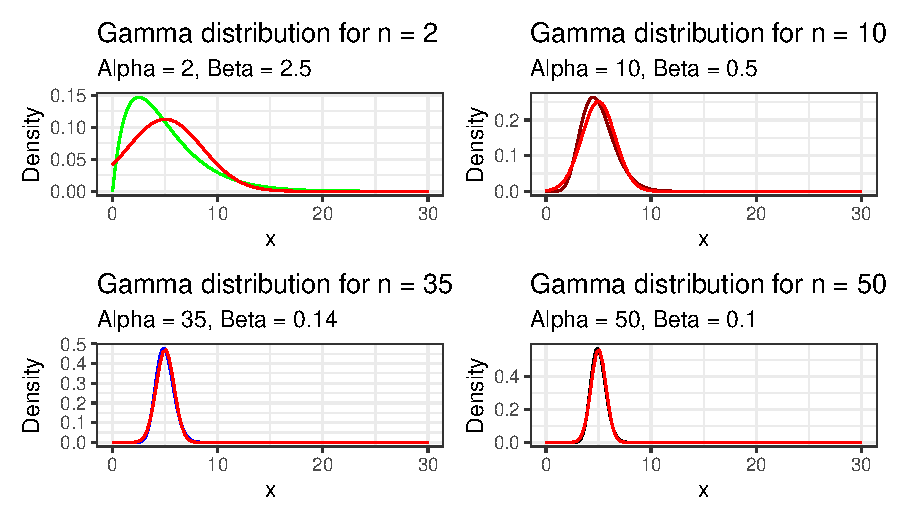
\includegraphics[width=\maxwidth]{figure/unnamed-chunk-9-1} 
\end{knitrout}
	  \item The Central Limit Theorem says that as $n$ increases, the sampling 
	  distribution of $\bar{Y}$ can be well approximated with a Gaussian 
	  distribution. Superimpose the approximate sampling distribution of $\bar{Y}$
	  for $n=2$, $n=10$, $n=35$, and $n=50$.
\begin{knitrout}
\definecolor{shadecolor}{rgb}{0.969, 0.969, 0.969}\color{fgcolor}\begin{kframe}
\begin{alltt}
\hlstd{plot1} \hlkwb{<-} \hlstd{plot1}\hlopt{+}
  \hlkwd{geom_function}\hlstd{(}\hlkwc{fun}\hlstd{=dnorm,} \hlkwc{args}\hlstd{=}\hlkwd{list}\hlstd{(}\hlkwc{mean}\hlstd{=}\hlnum{5}\hlstd{,} \hlkwc{sd}\hlstd{=}\hlnum{1}\hlstd{),}
                \hlkwc{color}\hlstd{=}\hlstr{"red"}\hlstd{)}

\hlstd{plot2} \hlkwb{<-} \hlstd{plot2}\hlopt{+}
  \hlkwd{geom_function}\hlstd{(}\hlkwc{fun}\hlstd{=dnorm,} \hlkwc{args}\hlstd{=}\hlkwd{list}\hlstd{(}\hlkwc{mean}\hlstd{=}\hlnum{5}\hlstd{,} \hlkwc{sd}\hlstd{=}\hlnum{1}\hlstd{),}
                \hlkwc{color}\hlstd{=}\hlstr{"red"}\hlstd{)}

\hlstd{plot3} \hlkwb{<-} \hlstd{plot3}\hlopt{+}
  \hlkwd{geom_function}\hlstd{(}\hlkwc{fun}\hlstd{=dnorm,} \hlkwc{args}\hlstd{=}\hlkwd{list}\hlstd{(}\hlkwc{mean}\hlstd{=}\hlnum{5}\hlstd{,} \hlkwc{sd}\hlstd{=}\hlnum{1}\hlstd{),}
                \hlkwc{color}\hlstd{=}\hlstr{"red"}\hlstd{)}

\hlstd{plot4} \hlkwb{<-} \hlstd{plot4}\hlopt{+}
  \hlkwd{geom_function}\hlstd{(}\hlkwc{fun}\hlstd{=dnorm,} \hlkwc{args}\hlstd{=}\hlkwd{list}\hlstd{(}\hlkwc{mean}\hlstd{=}\hlnum{5}\hlstd{,} \hlkwc{sd}\hlstd{=}\hlnum{1}\hlstd{),}
                \hlkwc{color}\hlstd{=}\hlstr{"red"}\hlstd{)}

\hlstd{(plot1}\hlopt{|}\hlstd{plot2)}\hlopt{/}\hlstd{(plot3}\hlopt{|}\hlstd{plot4)}
\end{alltt}


{\ttfamily\noindent\color{warningcolor}{\#\# Warning: Removed 700 row(s) containing missing values (geom\_path).}}

{\ttfamily\noindent\color{warningcolor}{\#\# Warning: Removed 700 row(s) containing missing values (geom\_path).}}

{\ttfamily\noindent\color{warningcolor}{\#\# Warning: Removed 700 row(s) containing missing values (geom\_path).}}

{\ttfamily\noindent\color{warningcolor}{\#\# Warning: Removed 700 row(s) containing missing values (geom\_path).}}\end{kframe}
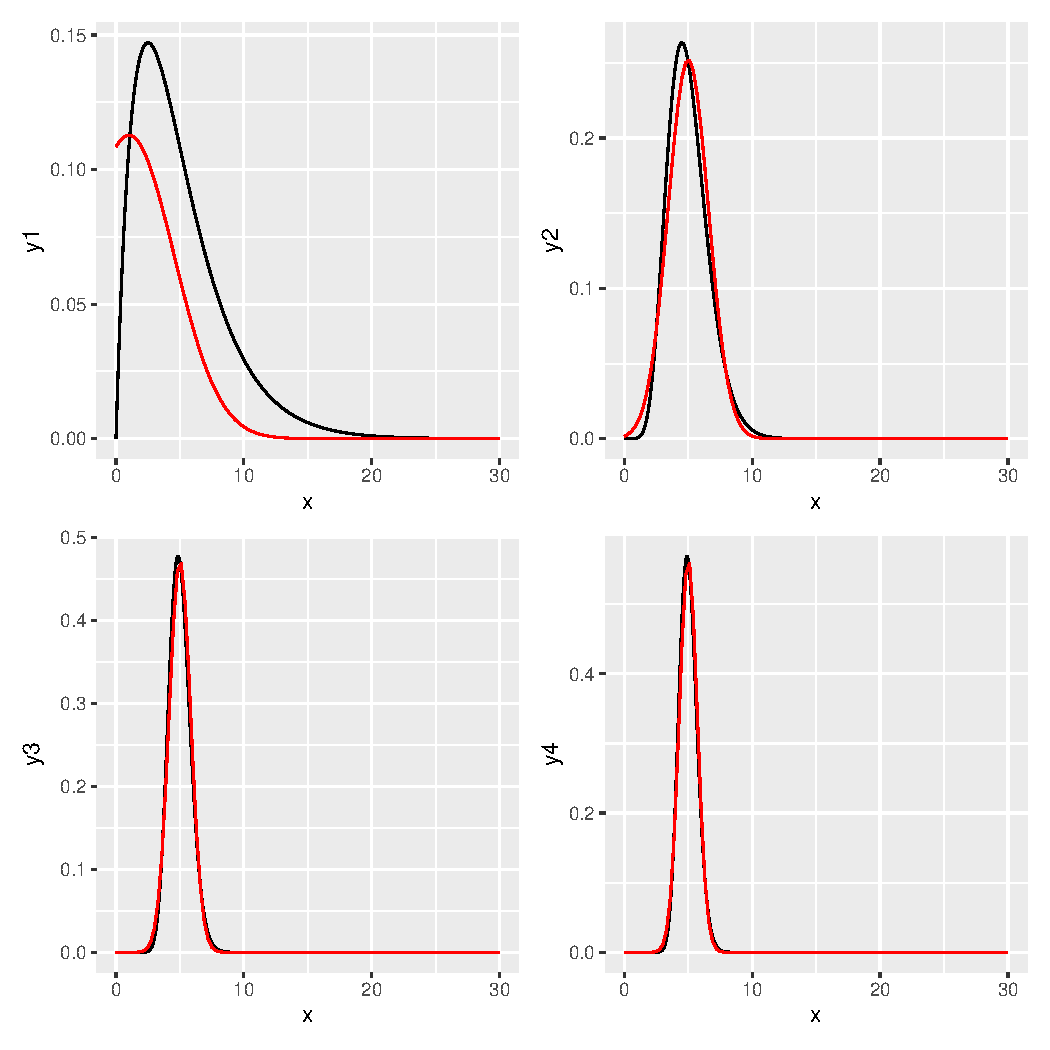
\includegraphics[width=\maxwidth]{figure/unnamed-chunk-10-1} 
\end{knitrout}
	  \item Find the probability that a randomly selected rat injected with the toxic substance
	  lives between 1 and 3 days.
\begin{knitrout}
\definecolor{shadecolor}{rgb}{0.969, 0.969, 0.969}\color{fgcolor}\begin{kframe}
\begin{alltt}
\hlcom{# P(x < 3) & P(x > 1) = 1-P(x<1)-P(x>3) = 1-P(x<=1)-(1-P(x>3))}
\hlnum{1}\hlopt{-}\hlkwd{pgamma}\hlstd{(}\hlkwc{q}\hlstd{=}\hlnum{1}\hlstd{,} \hlkwc{shape}\hlstd{=}\hlnum{1}\hlstd{,} \hlkwc{scale}\hlstd{=}\hlnum{1}\hlopt{/}\hlnum{0.2}\hlstd{)}\hlopt{-}\hlstd{(}\hlnum{1}\hlopt{-}\hlkwd{pgamma}\hlstd{(}\hlkwc{q}\hlstd{=}\hlnum{3}\hlstd{,} \hlkwc{shape}\hlstd{=}\hlnum{1}\hlstd{,} \hlkwc{scale}\hlstd{=}\hlnum{1}\hlopt{/}\hlnum{0.2}\hlstd{))}
\end{alltt}
\begin{verbatim}
## [1] 0.2699191
\end{verbatim}
\end{kframe}
\end{knitrout}
	  \item Find the exact probability, using the exact sampling distribution, that two randomly selected rats injected with the toxic substance live  between 1 and 3 days on average.
\begin{knitrout}
\definecolor{shadecolor}{rgb}{0.969, 0.969, 0.969}\color{fgcolor}\begin{kframe}
\begin{alltt}
\hlcom{# P(x < 3) & P(x > 1) = 1-P(x<1)-P(x>3) = 1-P(x<=1)-(1-P(x>3))}
\hlnum{1}\hlopt{-}\hlkwd{pgamma}\hlstd{(}\hlkwc{q}\hlstd{=}\hlnum{1}\hlstd{,} \hlkwc{shape}\hlstd{=}\hlnum{2}\hlstd{,} \hlkwc{scale}\hlstd{=}\hlnum{1}\hlopt{/}\hlstd{(}\hlnum{2}\hlopt{*}\hlnum{0.2}\hlstd{))}\hlopt{-}\hlstd{(}\hlnum{1}\hlopt{-}\hlkwd{pgamma}\hlstd{(}\hlkwc{q}\hlstd{=}\hlnum{3}\hlstd{,} \hlkwc{shape}\hlstd{=}\hlnum{2}\hlstd{,} \hlkwc{scale}\hlstd{=}\hlnum{1}\hlopt{/}\hlstd{(}\hlnum{2}\hlopt{*}\hlnum{0.2}\hlstd{)))}
\end{alltt}
\begin{verbatim}
## [1] 0.2758208
\end{verbatim}
\end{kframe}
\end{knitrout}
  \item Find the approximate probability, using the Central Limit Theorem, that two randomly 
	  selected rats injected with the toxic substance live between 1 and 3 days on average. Comment
	  on connection between the results and the assumptions of Central Limit Theorem.
\item Under what conditions would the approximate probability calculated in 
part (f) better match the exact probability in part (e)?
  \end{enumerate}
\newpage
%%%%%%%%%%%%%%%%%%%%%%%%%%%%%%%%%%%%%%%%%%%%%%%%%%%%%%%%%%%%%%%%%%%%%%%%%%%%%%%
%%%%%%%%%%%%%%%%%%%%%%%%%%%%%%%%%%%%%%%%%%%%%%%%%%%%%%%%%%%%%%%%%%%%%%%%%%%%%%%
%%%%%%%%%  Question 3
%%%%%%%%%%%%%%%%%%%%%%%%%%%%%%%%%%%%%%%%%%%%%%%%%%%%%%%%%%%%%%%%%%%%%%%%%%%%%%%
%%%%%%%%%%%%%%%%%%%%%%%%%%%%%%%%%%%%%%%%%%%%%%%%%%%%%%%%%%%%%%%%%%%%%%%%%%%%%%%
\item Below you will load and summarize a dataset 
  containing 575 observations of drug treatments. The data includes the following
  \begin{itemize}
    \item ID --	Identification Code	(1 - 575)
    \item AGE	-- Age at Enrollment	(Years)
    \item BECK -- Beck Depression Score	(0.000 - 54.000)
    \item HC --	Heroin/Cocaine Use During	3 Months Prior to Admission (1 = Heroin
    \& Cocaine; 2 = Heroin Only, 3 = Cocaine Only; 4 = Neither Heroin nor Cocaine)
    \item IV -- History of IV Drug Use	(1 = Never; 2 = Previous; 3 = Recent)
    \item IV3	-- Recent IV use	(1 = Yes; 0 = No)
    \item NDT -- Number of Prior Drug Treatments (0 - 40)
    \item RACE -- Subject's Race	(0 = White; 1 = Non-White)
\item TREAT -- Treatment Randomization (0 = Short Assignment;	1 = Long Assignment)
\item SITE -- Treatment Site (0 = A; 1 = B)
\item LEN.T	-- Length of Stay in Treatment (Days Admission Date to Exit Date)	
\item TIME -- Time to Drug Relapse (Days Measured from Admission Date)
\item CENSOR -- Event for Treating Lost to Follow-Up as Returned to Drugs 
(1 = Returned to Drugs or Lost to Follow-Up; 0 = Otherwise)
\item etc.
\end{itemize}
\begin{enumerate} %this begins a lettered enumerate so I can ask more 
%than one question in a question.
\item Load the data provided in the ``quantreg" package for \texttt{R} \citep{quantreg}.
\begin{knitrout}
\definecolor{shadecolor}{rgb}{0.969, 0.969, 0.969}\color{fgcolor}\begin{kframe}
\begin{alltt}
\hlkwd{library}\hlstd{(}\hlstr{"quantreg"}\hlstd{)}
\hlkwd{data}\hlstd{(}\hlstr{"uis"}\hlstd{)}
\end{alltt}
\end{kframe}
\end{knitrout}
\item Is there evidence that patients receiving drug treatments are at least mildly depressed
on average? That is, is there evidence that the average BECK depression score is greater
than 13, $\mu>13$?
    \begin{enumerate}
      \item What is the null hypothesis for this test?\\
      \textbf{Solution:} $H_{0}: \mu=13$
      \item What is the alternative hypothesis for this test?\\
      \textbf{Solution:} $H_{a}: \mu>13$
      \item What is the sample mean BECK score for these data?\\
      \textbf{Solution:}
\begin{knitrout}
\definecolor{shadecolor}{rgb}{0.969, 0.969, 0.969}\color{fgcolor}\begin{kframe}
\begin{alltt}
\hlstd{mu} \hlkwb{<-} \hlkwd{mean}\hlstd{(uis}\hlopt{$}\hlstd{BECK)}
\hlkwd{paste}\hlstd{(}\hlstr{"The mean of BECK is"}\hlstd{,} \hlkwd{mean}\hlstd{(mu))}
\end{alltt}
\begin{verbatim}
## [1] "The mean of BECK is 17.367427826087"
\end{verbatim}
\end{kframe}
\end{knitrout}
      \item What is the test statistics for this test?\\
      \textbf{Solution:} Mean would be our test statistics.
\begin{knitrout}
\definecolor{shadecolor}{rgb}{0.969, 0.969, 0.969}\color{fgcolor}\begin{kframe}
\begin{alltt}
\hlkwd{mean}\hlstd{(uis}\hlopt{$}\hlstd{BECK)}
\end{alltt}
\begin{verbatim}
## [1] 17.36743
\end{verbatim}
\begin{alltt}
\hlkwd{median}\hlstd{(uis}\hlopt{$}\hlstd{BECK)}
\end{alltt}
\begin{verbatim}
## [1] 17
\end{verbatim}
\begin{alltt}
\hlcom{#Mean is basically equal to median, so we don't really care. c:}
\end{alltt}
\end{kframe}
\end{knitrout}
      \item At what value of $\bar{X}$ does the rejection region start for $\alpha=0.05$?\\
      
      \begin{align*}
	se &= \frac{s}{\sqrt{n}} \tag{Formula for finding t-value}\\
	t &= \frac{\bar{X}-\mu}{se} \tag{Formula for finding t-value}\\
	\bar{X} &= t*se + \mu \tag{Solving for $\bar{X}$}
	    \end{align*}
\begin{knitrout}
\definecolor{shadecolor}{rgb}{0.969, 0.969, 0.969}\color{fgcolor}\begin{kframe}
\begin{alltt}
\hlstd{n}\hlkwb{<-}\hlkwd{nrow}\hlstd{(uis)}
\hlstd{se} \hlkwb{=} \hlkwd{sd}\hlstd{(uis}\hlopt{$}\hlstd{BECK)}\hlopt{/}\hlkwd{sqrt}\hlstd{(n)}
\hlstd{(value}\hlkwb{<-}\hlstd{(}\hlkwd{qt}\hlstd{(}\hlnum{.95}\hlstd{, n}\hlopt{-}\hlnum{1}\hlstd{)}\hlopt{*}\hlstd{se)}\hlopt{+}\hlstd{mu)}
\end{alltt}
\begin{verbatim}
## [1] 18.00866
\end{verbatim}
\end{kframe}
\end{knitrout}
      \item What is the p value for this test?
\begin{knitrout}
\definecolor{shadecolor}{rgb}{0.969, 0.969, 0.969}\color{fgcolor}\begin{kframe}
\begin{alltt}
\hlstd{n}\hlkwb{=}\hlkwd{nrow}\hlstd{(uis)}
\hlstd{tstat} \hlkwb{<-} \hlkwd{t.test}\hlstd{(}\hlkwc{x}\hlstd{=uis}\hlopt{$}\hlstd{BECK,}
       \hlkwc{mu} \hlstd{=} \hlnum{13}\hlstd{,}
       \hlkwc{alternative} \hlstd{=} \hlstr{"greater"}\hlstd{)}

\hlstd{tstat}\hlopt{$}\hlstd{p.value}
\end{alltt}
\begin{verbatim}
## [1] 7.412123e-27
\end{verbatim}
\end{kframe}
\end{knitrout}
      \item Graph the results of this test.
\begin{knitrout}
\definecolor{shadecolor}{rgb}{0.969, 0.969, 0.969}\color{fgcolor}\begin{kframe}
\begin{alltt}
\hlstd{ggdat} \hlkwb{<-} \hlkwd{data.frame}\hlstd{(}\hlkwc{t}\hlstd{=}\hlkwd{seq}\hlstd{(}\hlopt{-}\hlnum{5}\hlstd{,}\hlnum{5}\hlstd{,}\hlkwc{length}\hlstd{=}\hlnum{500}\hlstd{))}\hlopt
  \hlkwd{mutate}\hlstd{(}\hlkwc{f}\hlstd{=}\hlkwd{dt}\hlstd{(}\hlkwc{x}\hlstd{=t,} \hlkwc{df}\hlstd{=n}\hlopt{-}\hlnum{1}\hlstd{))}

\hlkwd{ggplot}\hlstd{(}\hlkwc{data}\hlstd{=ggdat,} \hlkwd{aes}\hlstd{(}\hlkwc{x}\hlstd{=t,} \hlkwc{y}\hlstd{=f))}\hlopt{+}
  \hlkwd{geom_line}\hlstd{()} \hlopt{+}
  \hlkwd{geom_hline}\hlstd{(}\hlkwc{yintercept}\hlstd{=}\hlnum{0}\hlstd{)}\hlopt{+}
  \hlkwd{geom_point}\hlstd{(}\hlkwd{aes}\hlstd{(}\hlkwc{x}\hlstd{=tstat}\hlopt{$}\hlstd{statistic,} \hlkwc{y}\hlstd{=}\hlnum{0}\hlstd{),} \hlkwc{color}\hlstd{=}\hlstr{"red"}\hlstd{)}\hlopt{+}
  \hlkwd{geom_vline}\hlstd{(}\hlkwc{xintercept}\hlstd{=}\hlkwd{qt}\hlstd{(}\hlkwc{p}\hlstd{=}\hlnum{0.95}\hlstd{,} \hlkwc{df}\hlstd{=n}\hlopt{-}\hlnum{1}\hlstd{),}
             \hlkwc{linetype}\hlstd{=}\hlstr{"dashed"}\hlstd{,} \hlkwc{color}\hlstd{=}\hlstr{"red"}\hlstd{)}\hlopt{+}
  \hlkwd{annotate}\hlstd{(}\hlstr{"text"}\hlstd{,} \hlkwc{x}\hlstd{=}\hlnum{1.2}\hlopt{*}\hlkwd{qt}\hlstd{(}\hlkwc{p}\hlstd{=}\hlnum{0.95}\hlstd{,} \hlkwc{df}\hlstd{=n}\hlopt{-}\hlnum{1}\hlstd{),} \hlkwc{y}\hlstd{=}\hlnum{0.30}\hlstd{,}
           \hlkwc{label}\hlstd{=}\hlstr{"Rejection Region"}\hlstd{,} \hlkwc{angle}\hlstd{=}\hlstr{"270"}\hlstd{,}
           \hlkwc{color}\hlstd{=}\hlstr{"red"}\hlstd{)}\hlopt{+}
  \hlkwd{annotate}\hlstd{(}\hlstr{"text"}\hlstd{,} \hlkwc{x}\hlstd{=tstat}\hlopt{$}\hlstd{statistic}\hlopt{-}\hlnum{1.8}\hlstd{,} \hlkwc{y}\hlstd{=}\hlnum{0.02}\hlstd{,}
           \hlkwc{label}\hlstd{=}\hlstr{"P-value = 7.41 * 10^-27"}\hlstd{,}
           \hlkwc{size}\hlstd{=}\hlnum{3}\hlstd{)}
\end{alltt}
\end{kframe}
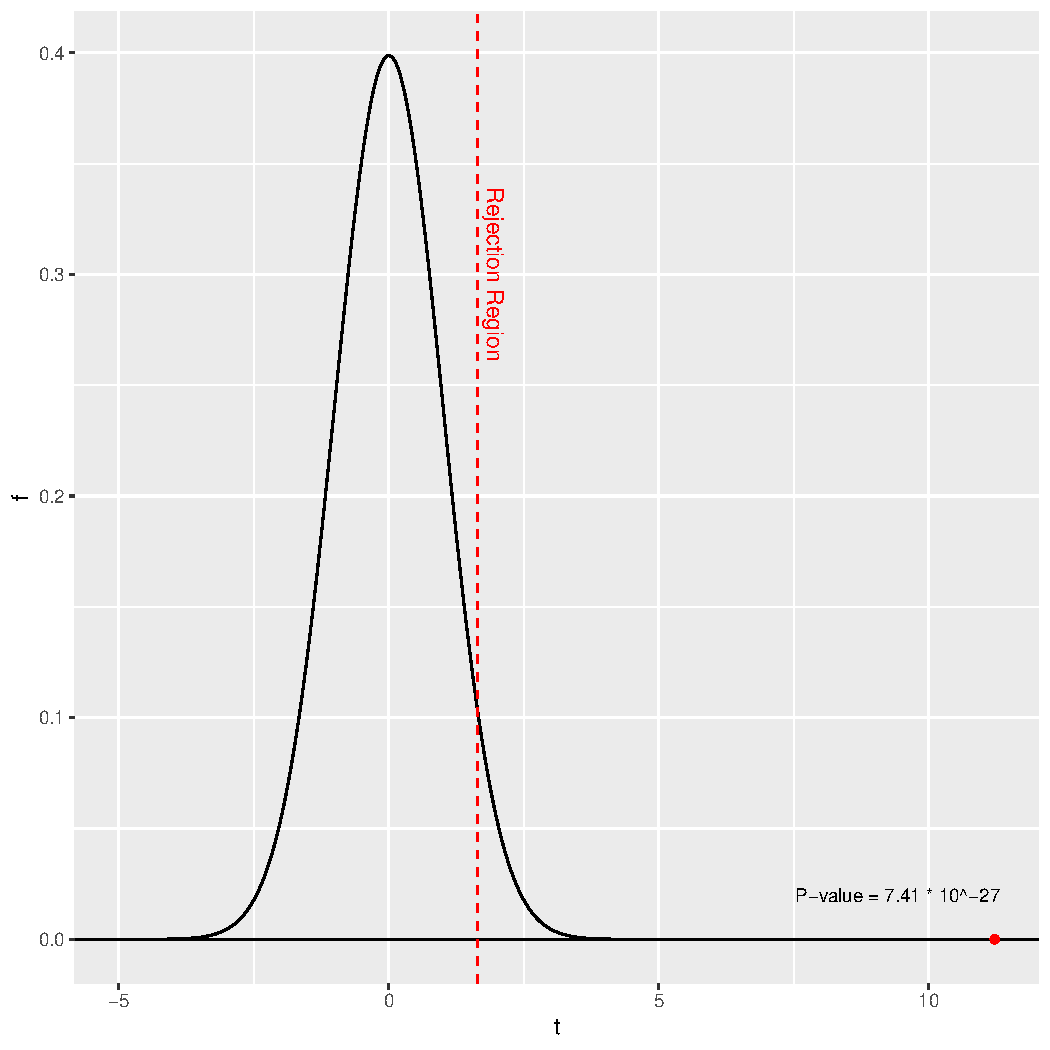
\includegraphics[width=\maxwidth]{figure/unnamed-chunk-18-1} 
\end{knitrout}
      \item Report a 95\% confidence interval for the average BECK depression score
and interpret it in the context of this question.
\begin{knitrout}
\definecolor{shadecolor}{rgb}{0.969, 0.969, 0.969}\color{fgcolor}\begin{kframe}
\begin{alltt}
\hlstd{ci}\hlkwb{<-}\hlkwd{t.test}\hlstd{(}\hlkwc{x}\hlstd{=uis}\hlopt{$}\hlstd{BECK,}
       \hlkwc{alternative} \hlstd{=} \hlstr{"two.sided"}\hlstd{)}

\hlkwd{paste}\hlstd{(}\hlstr{"The confidence interval is ["}\hlstd{, ci}\hlopt{$}\hlstd{conf.int[}\hlnum{1}\hlstd{],} \hlstr{", "}\hlstd{,}
      \hlstd{ci}\hlopt{$}\hlstd{conf.int[}\hlnum{2}\hlstd{],}\hlstr{"]"}\hlstd{,} \hlkwc{sep}\hlstd{=}\hlstr{""}\hlstd{)}
\end{alltt}
\begin{verbatim}
## [1] "The confidence interval is [16.6029755170859, 18.131880135088]"
\end{verbatim}
\end{kframe}
\end{knitrout}
    \end{enumerate}
\item Is there a significant difference in the length of stay in treatment by 
    treatment site?\\
\textbf{Solution:}
\begin{align*}
H_{0}&:\mu_{0}=\mu{1}\\
H_{a}&:\mu_{0}\neq\mu{1}
\end{align*}
\begin{knitrout}
\definecolor{shadecolor}{rgb}{0.969, 0.969, 0.969}\color{fgcolor}\begin{kframe}
\begin{alltt}
\hlstd{res} \hlkwb{<-} \hlkwd{t.test}\hlstd{(uis}\hlopt{$}\hlstd{LEN.T} \hlopt{~} \hlstd{uis}\hlopt{$}\hlstd{SITE,} \hlkwc{data} \hlstd{= uis,} \hlkwc{var.equal} \hlstd{=} \hlnum{TRUE}\hlstd{)}
\hlstd{res}
\end{alltt}
\begin{verbatim}
## 
## 	Two Sample t-test
## 
## data:  uis$LEN.T by uis$SITE
## t = -7.8446, df = 573, p-value = 2.137e-14
## alternative hypothesis: true difference in means is not equal to 0
## 95 percent confidence interval:
##  -65.03172 -38.98756
## sample estimates:
## mean in group 0 mean in group 1 
##         84.9275        136.9371
\end{verbatim}
\end{kframe}
\end{knitrout}
  \end{enumerate}
  \newpage
%%%%%%%%%%%%%%%%%%%%%%%%%%%%%%%%%%%%%%%%%%%%%%%%%%%%%%%%%%%%%%%%%%%%%%%%%%%%%%%
%%%%%%%%%%%%%%%%%%%%%%%%%%%%%%%%%%%%%%%%%%%%%%%%%%%%%%%%%%%%%%%%%%%%%%%%%%%%%%%
%%%%%%%%%  Question 4
%%%%%%%%%%%%%%%%%%%%%%%%%%%%%%%%%%%%%%%%%%%%%%%%%%%%%%%%%%%%%%%%%%%%%%%%%%%%%%%
%%%%%%%%%%%%%%%%%%%%%%%%%%%%%%%%%%%%%%%%%%%%%%%%%%%%%%%%%%%%%%%%%%%%%%%%%%%%%%%
\item Below you will load and summarize a dataset containing 53 observations of prostate cance patients.
In this research, a number of possible predictor variables were measured before surgery. The patients then 
had surgery to determine nodal involvement. 
  \begin{itemize}
    \item r -- Nodal Involvement (0=No, 1=Yes)
    \item aged	-- Age Group (0=Less than 60, 1=At least 60)
    \item stage -- Palpitation Result Severity (0=Less severe, 1=More severe)
    \item grade -- Biopsy Result Severity (0=Less severe, 1=More severe)
    \item xray -- X-ray Result Severity (0=Less severe, 1=More severe)
    \item acid -- the level of acid phosphatase in the blood serum
\end{itemize}
The treatment strategy for a patient diagnosed with cancer of the prostate depend highly on whether the cancer has spread to the surrounding lymph nodes (nodal involvement). It is common to operate on the patient to get samples from the nodes which can then be analysed under a microscope.

\begin{enumerate} %this begins a lettered enumerate so I can ask more 
%than one question in a question.
\item Load the data provided in the ``boot" package for \texttt{R} \citep{boot}.
\begin{knitrout}
\definecolor{shadecolor}{rgb}{0.969, 0.969, 0.969}\color{fgcolor}\begin{kframe}
\begin{alltt}
\hlkwd{library}\hlstd{(}\hlstr{"boot"}\hlstd{)}
\hlkwd{data}\hlstd{(}\hlstr{"nodal"}\hlstd{)}
\end{alltt}
\end{kframe}
\end{knitrout}
\item Is there evidence that less than half of prostate cancer patients have nodal involvment?
    \begin{enumerate}
      \item What is the null hypothesis for this test?\\
      \textbf{Solution:}  $H_{0}: \hat{P}=0.5$
      \item What is the alternative hypothesis for this test?\\
      \textbf{Solution:}  $H_{0}: \hat{P}\neq0.5$
      \item What is the sample proportion of patients with nodal involvement for these data?\\
      \textbf{Solution:} Something
\begin{knitrout}
\definecolor{shadecolor}{rgb}{0.969, 0.969, 0.969}\color{fgcolor}\begin{kframe}
\begin{alltt}
\hlkwd{table}\hlstd{(nodal}\hlopt{$}\hlstd{r)[}\hlnum{2}\hlstd{]}\hlopt{/}\hlkwd{nrow}\hlstd{(nodal)} \hlcom{#.37%}
\end{alltt}
\begin{verbatim}
##         1 
## 0.3773585
\end{verbatim}
\end{kframe}
\end{knitrout}
      \item What is the test statistics for this test?\\
      \textbf{Solution:} Z-value 
      \item At what value of $\hat{P}$ does the rejection region start for $\alpha=0.05$?
      \begin{align*}
      z &= \frac{\hat{p}-p_{0}}{\sqrt{\frac{p_{0}(1-p_{0})}{n}}}\\
      \hat{p} &= \frac{\sqrt{n}z\sqrt{p_{0}(1-p_{0})}}{n} + p_{0}
      \end{align*}
\begin{knitrout}
\definecolor{shadecolor}{rgb}{0.969, 0.969, 0.969}\color{fgcolor}\begin{kframe}
\begin{alltt}
\hlstd{p0} \hlkwb{<-} \hlnum{0.5}
\hlstd{phat} \hlkwb{<-} \hlkwd{table}\hlstd{(nodal}\hlopt{$}\hlstd{r)[}\hlnum{2}\hlstd{]}\hlopt{/}\hlkwd{nrow}\hlstd{(nodal)}
\hlstd{n} \hlkwb{<-} \hlkwd{nrow}\hlstd{(nodal)}
\hlstd{z1} \hlkwb{<-} \hlkwd{qt}\hlstd{(}\hlnum{.975}\hlstd{, n}\hlopt{-}\hlnum{1}\hlstd{)}
\hlstd{z2} \hlkwb{<-} \hlopt{-}\hlstd{z1}

\hlstd{(}\hlkwd{sqrt}\hlstd{(n)}\hlopt{*}\hlstd{z1}\hlopt{*}\hlkwd{sqrt}\hlstd{(p0}\hlopt{*}\hlstd{(}\hlnum{1}\hlopt{-}\hlstd{p0)))}\hlopt{/}\hlstd{(n)} \hlopt{+} \hlstd{p0} \hlcom{#for upper bound}
\end{alltt}
\begin{verbatim}
## [1] 0.6378171
\end{verbatim}
\begin{alltt}
\hlstd{(}\hlkwd{sqrt}\hlstd{(n)}\hlopt{*}\hlstd{z2}\hlopt{*}\hlkwd{sqrt}\hlstd{(p0}\hlopt{*}\hlstd{(}\hlnum{1}\hlopt{-}\hlstd{p0)))}\hlopt{/}\hlstd{(n)} \hlopt{+} \hlstd{p0} \hlcom{#for lower bound}
\end{alltt}
\begin{verbatim}
## [1] 0.3621829
\end{verbatim}
\end{kframe}
\end{knitrout}
      \item What is the p value for this test?
\begin{knitrout}
\definecolor{shadecolor}{rgb}{0.969, 0.969, 0.969}\color{fgcolor}\begin{kframe}
\begin{alltt}
\hlstd{zAns} \hlkwb{<-} \hlstd{(phat}\hlopt{-}\hlstd{p0)}\hlopt{/}\hlkwd{sqrt}\hlstd{((p0}\hlopt{*}\hlstd{(}\hlnum{1}\hlopt{-}\hlstd{p0))}\hlopt{/}\hlstd{(n))}
\hlstd{zAns}
\end{alltt}
\begin{verbatim}
##         1 
## -1.785687
\end{verbatim}
\end{kframe}
\end{knitrout}
      \item Graph the results of this test.
\begin{knitrout}
\definecolor{shadecolor}{rgb}{0.969, 0.969, 0.969}\color{fgcolor}\begin{kframe}
\begin{alltt}
\hlstd{ggdat} \hlkwb{<-} \hlkwd{data.frame}\hlstd{(}\hlkwc{t}\hlstd{=}\hlkwd{seq}\hlstd{(}\hlopt{-}\hlnum{5}\hlstd{,}\hlnum{5}\hlstd{,}\hlkwc{length}\hlstd{=}\hlnum{500}\hlstd{))}\hlopt
  \hlkwd{mutate}\hlstd{(}\hlkwc{f}\hlstd{=}\hlkwd{dt}\hlstd{(}\hlkwc{x}\hlstd{=t,} \hlkwc{df}\hlstd{=n}\hlopt{-}\hlnum{1}\hlstd{))}

\hlkwd{ggplot}\hlstd{(}\hlkwc{data}\hlstd{=ggdat,} \hlkwd{aes}\hlstd{(}\hlkwc{x}\hlstd{=t,} \hlkwc{y}\hlstd{=f))}\hlopt{+}
  \hlkwd{geom_line}\hlstd{()} \hlopt{+}
  \hlkwd{geom_hline}\hlstd{(}\hlkwc{yintercept}\hlstd{=}\hlnum{0}\hlstd{)}\hlopt{+}
  \hlkwd{geom_point}\hlstd{(}\hlkwd{aes}\hlstd{(}\hlkwc{x}\hlstd{=zAns,} \hlkwc{y}\hlstd{=}\hlnum{0}\hlstd{),} \hlkwc{color}\hlstd{=}\hlstr{"red"}\hlstd{)}\hlopt{+}
  \hlkwd{geom_vline}\hlstd{(}\hlkwc{xintercept}\hlstd{=}\hlkwd{qt}\hlstd{(}\hlkwc{p}\hlstd{=}\hlnum{0.975}\hlstd{,} \hlkwc{df}\hlstd{=n}\hlopt{-}\hlnum{1}\hlstd{),}
              \hlkwc{linetype}\hlstd{=}\hlstr{"dashed"}\hlstd{,} \hlkwc{color}\hlstd{=}\hlstr{"red"}\hlstd{)}\hlopt{+}
  \hlkwd{geom_vline}\hlstd{(}\hlkwc{xintercept}\hlstd{=}\hlkwd{qt}\hlstd{(}\hlkwc{p}\hlstd{=}\hlnum{0.025}\hlstd{,} \hlkwc{df}\hlstd{=n}\hlopt{-}\hlnum{1}\hlstd{),}
              \hlkwc{linetype}\hlstd{=}\hlstr{"dashed"}\hlstd{,} \hlkwc{color}\hlstd{=}\hlstr{"red"}\hlstd{)}
\end{alltt}
\end{kframe}
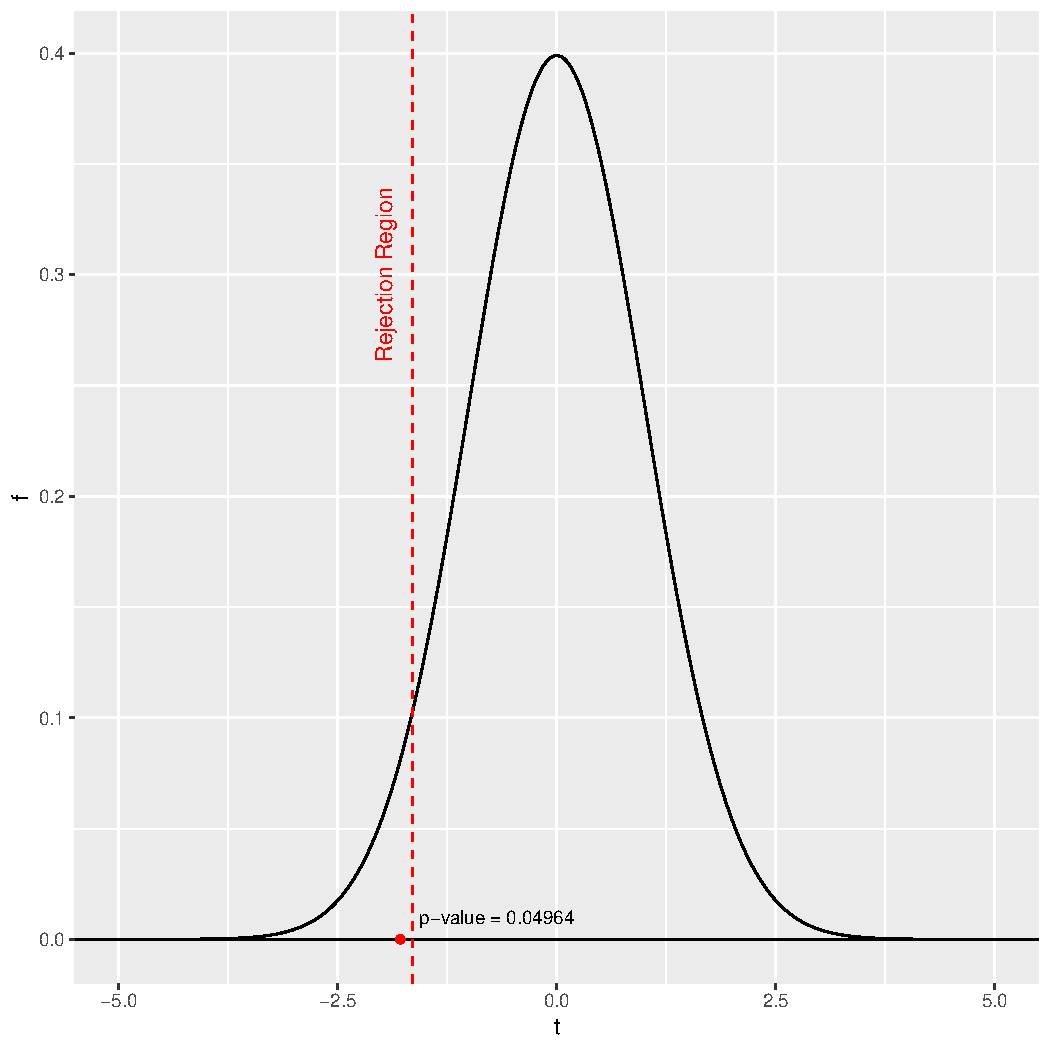
\includegraphics[width=\maxwidth]{figure/unnamed-chunk-25-1} 
\end{knitrout}
      \item Report a 95\% confidence interval for the proportion of prostate cancer patients with nodal involvement and interpret it in the context of this question.
\begin{knitrout}
\definecolor{shadecolor}{rgb}{0.969, 0.969, 0.969}\color{fgcolor}\begin{kframe}
\begin{alltt}
\hlcom{#no clue}
\end{alltt}
\end{kframe}
\end{knitrout}
    \end{enumerate}
    \item Clearly, it would be preferable if an accurate assessment of nodal involvement could be made without surgery. Is there a significant difference in the nodal involvement of patients with any of the severity indicators?
  \end{enumerate}
\end{enumerate}
%%%%%%%%%%%%%%%%%%%%%%%%%%%%%%%%%%%%%%%%%%%%%%%%%%%%%%%%%%%%%%%%%%%%%%%%%%%%%%%
%%%%%%%%%%%%%%%%%%%%%%%%%%%%%%%%%%%%%%%%%%%%%%%%%%%%%%%%%%%%%%%%%%%%%%%%%%%%%%%
%%%%%%%%%  Bibliography
%%%%%%%%%%%%%%%%%%%%%%%%%%%%%%%%%%%%%%%%%%%%%%%%%%%%%%%%%%%%%%%%%%%%%%%%%%%%%%%
%%%%%%%%%%%%%%%%%%%%%%%%%%%%%%%%%%%%%%%%%%%%%%%%%%%%%%%%%%%%%%%%%%%%%%%%%%%%%%%
\newpage
\noindent \textbf{Bonus 1:} Use the gganimate package \citep{gganimate} for \texttt{R} to create a plot that demonstrates the Central Limit Theorem for the Poisson, Binomial, Exponential, and Gaussian distributions in a $2\times 2$ grid as \href{https://moodle.colgate.edu/mod/forum/discuss.php?d=127682}{here}.\\

Note that we can't add GIFs to the .pdf document, so you'll have to email me your code for this part. You'll find \texttt{  transition\_time()} helpful for creating your animation and \texttt{gganimate\_save()} helpful for saving your animation. \vspace{2em}\\


\noindent \textbf{Bonus 2:} Compare the effectiveness of the $t$-interval with the bootstrap interval. In a loop, generate 1000 datasets, evaluate a $t$ and bootstrapping confidence interval for each set of data, and track whether you've captured the true population mean. An effective answer here would evaluate this several times varying sample size and the data generating distribution.

\newpage
\bibliography{bib}
\end{document}
